\vssub
\subsection{~Spatial and temporal tracking of wave systems} \label{sub:num_track}
\conthead{IFP Swan}{Van der Westhuysen, Hanson, Devaliere}

\noindent
The spectral partitioning procedure described above is carried out within the
spectral space, independently at each geographical grid point. As a result,
there is no coherence between the identified partitions over geographical
space and in time. Following \cite{art:VMH97}, \cite{art:HP01} and
\cite{pro:DHL09}, a spatial correlation step is therefore applied.  This is
done by means of an outwardly running spiral, originating at an arbitrary
point (typically the center) inside the computational domain.
Figure~\ref{fig:wavetrack} presents an example of such a tracking spiral on a
regular computational grid over a coastal domain featuring landmass. At the
spiral origin (location~1), each spectral partition is assigned an initial
system index. The spatial correlation is then determined for each subsequent
geographical location (2, 3, 4, ...) moving outward along the spiral.  At each
new geographical location, the peak period $T_\mathrm{p}$, peak direction
$\theta_\mathrm{p}$ and significant wave height $H_\mathrm{m0}$ of each of its
spectral partitions are correlated with the spatial means
$\tilde{T}^\mathrm{n}_{\mathrm{p},i}$,
$\tilde{\theta}^\mathrm{n}_{\mathrm{p},i}$ and
$\tilde{H}^\mathrm{n}_{\mathrm{m0},i}$ of the corresponding parameters at its
neighboring geographical grid points (indicated by the superscript
$\mathrm{n}$) previously assigned a system $i$. the partition at the present
grid point is assigned to the neighboring system $i$ that minimizes the
following Goodness-of-Fit (GoF) function:

\begin{figure} \begin{center}
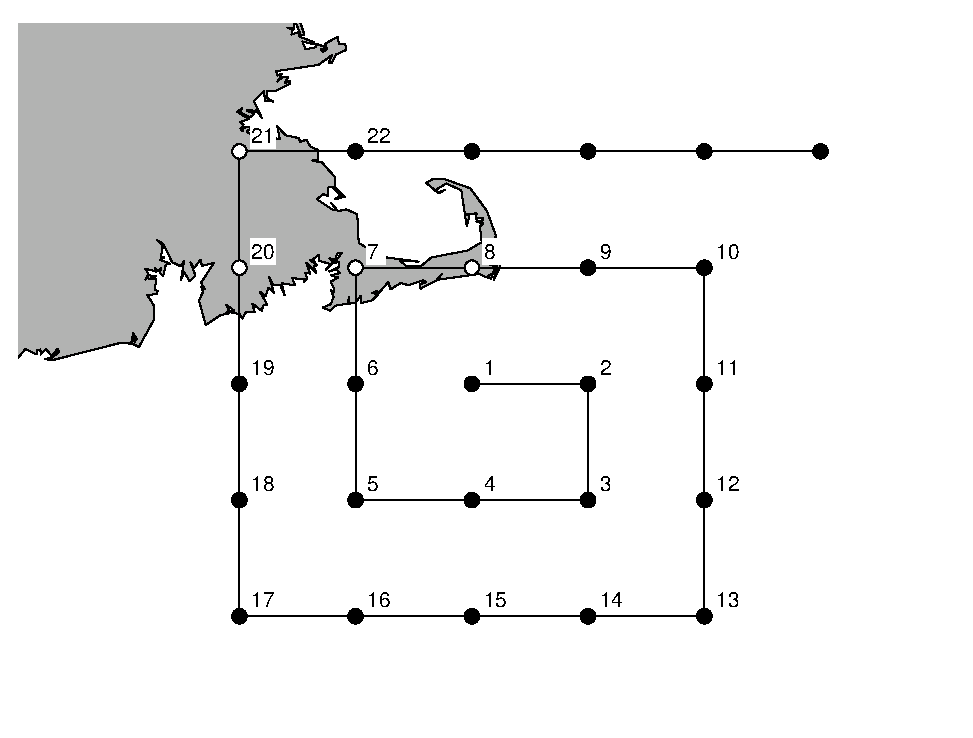
\epsfig{file=./num/wavetrack.eps,width=3.5in}
\caption{Example of a tracking spiral on a regular computational grid 
over a coastal domain featuring landmass (shaded). Black dots indicate 
active grid points and white dots indicate inactive (dry) grid points.}
         \label{fig:wavetrack} \botline
\end{center}
\end{figure}

\begin{equation}
    GoF_{i} = {\left( \frac{T_\mathrm{p} - \tilde{T}^\mathrm{n}_{\mathrm{p},i}}{\Delta T_\mathrm{n}} \right)}^2 + 
                     {\left( \frac{\theta_\mathrm{p} - \tilde{\theta}^\mathrm{n}_{\mathrm{p},i}}{\Delta\theta_\mathrm{n}} \right)}^2 +
                     {\left( \frac{H_\mathrm{m0} - \tilde{H}^\mathrm{n}_{\mathrm{m0},i}}{\Delta H_\mathrm{n}} \right)}^2\ \ ,
\label{eq:grdgof}
\end{equation} 

\noindent
where $\Delta T_\mathrm{n}$, $\Delta\theta_\mathrm{n}$ and $\Delta
H_\mathrm{n}$ are combining criteria \citep{art:WHD13}. If either of the first
two terms on the right hand side of (\ref{eq:grdgof}) exceed unity for the
closest match, the difference is considered too great and a new wave system is
assigned to that partition. Here, the search range for neighboring points is
set at 1, so that a maximum of four previously-associated neighbors can be
found (e.g. location 15 will have the previously processed neighbors 3, 4, 5
and 14). In some cases, iterative combining is required.

The next step is to correlate these wave systems over time. Each system $i$ at
the current time level $t$ is associated with its closest match amongst the
systems $j$ at the previous time level $(t-1)$. Three characteristics of the
wave systems are considered in this process, namely: (i) the spatial mean peak
wave period over the system, $\tilde{T}^\mathrm{s}_{\mathrm{p},t,i}$, with
$\mathrm{s}$ denoting the system mean, (ii) the spatial mean peak wave
direction, $\tilde{\theta}^\mathrm{s}_{\mathrm{p},t,i}$ and (iii) the number
of overlapping grid points between the two systems in geographical space
$\cap_{i,j}$. These characteristics are combined to form the following
GoF function:

\begin{equation}
    GoF_{i,j} = {\left( \frac{\tilde{T}^\mathrm{s}_{\mathrm{p},t,i} - \tilde{T}^\mathrm{s}_{\mathrm{p},t-1,j}}{\Delta T_\mathrm{s}} \right)}^2 + 
                       {\left( \frac{\tilde{\theta}^\mathrm{s}_{\mathrm{p},t,i} - \tilde{\theta}^\mathrm{s}_{\mathrm{p},t-1,j}}{\Delta\theta_\mathrm{s}} \right)}^2 +
                       {\left( \frac{N_{t-1,j} - \cap_{i,j}}{0.5N_{t-1,j}} \right)}^2\ \ ,
\label{eq:timegof}
\end{equation} 

\noindent
where $\Delta T_\mathrm{s}$ and $\Delta\theta_\mathrm{s}$ are combining
criteria, and $N$ is the total number of grid points in a system, see
\cite{art:WHD13}. In order to focus the tracking process on high-energy
regions in the wave field, the spatial mean period and peak direction values
of each system are weighted with the square of the significant wave
height. System $i$ at the current time level $t$ is assigned the system $j$
from the previous time level $(t-1)$ that minimizes (\ref{eq:timegof}). If any
of the three terms on the right hand side of (\ref{eq:timegof}) exceed unity
for the system that minimizes (\ref{eq:timegof}), a new system number is
assigned. For the last term, this implies a minimum spatial overlap
requirement, arbitrarily set at 50\%. This term mostly has an impact over
basin scale domains, where systems are typically smaller than the
computational area. In order to improve robustness, the details of identified
systems are stored for five time levels, after which the system association is
released.



